\section{Decision-Tree Induction}

\begin{frame}{Decision-Tree: An Example}
	\begin{columns}
		\begin{column}{0.38\textwidth}
			\vspace{-3cm}
			\begin{itemize}
				\item \textbf{Training dataset: buys\_computer.}\newline
				      The dataset follows an example of Quinlan's ID3.
				\item \textbf{Resulting tree:}\\[0.1cm]
			\end{itemize}
			\centering
			\begin{tikzpicture}[
		overlay,
		remember picture,
		>=latex,
		thick,
		node/.style={
				draw=faugray,
				rounded corners=.25em,
				fill=faugray!62,
				text depth=0.2em
			},
		leaf/.style={
				draw,
				rounded corners=.7em,
				text depth=0.2em
			},
		branch/.style={
				fill=white,
				font=\ttfamily\scriptsize,
				rounded corners=.7em,
				text depth=0.2em
			}
	]
	\node[node] at (0,0) (age) {age?};
	\node[leaf,text=faugreen,below=6.2em of age] (age-yes) {yes};

	\node[node,below left=2em and 1.5em of age] (student) {student?};
	\node[leaf,text=faured,below right=2.5em and -1em of student] (student-no) {no};
	\node[leaf,text=faugreen,below left=2.5em and -1em of student] (student-yes) {yes};

	\node[node,below right=2em and .6em of age] (credit-rating) {credit rating?};
	\node[leaf,text=faured,below left=2.5em and -2em of credit-rating] (credit-no) {no};
	\node[leaf,text=faugreen,below right=2.5em and -2em of credit-rating] (credit-yes) {yes};

	\draw (age.south) -- (age-yes.north);
	\node[branch,below=4em of age.north] {31\dots 40};

	\draw[rounded corners=5pt]
	(age.south) -- ($(age.south) + (0,-1em)$) --
	($(student.north) + (0,1em)$) -- (student.north);
	\node[branch,above=1em of student.north] {$\leq$30};

	\path[draw,rounded corners=5pt]
	(age.south) -- ($(age.south) + (0,-1em)$) --
	($(credit-rating.north) + (0,1em)$) -- (credit-rating.north);
	\node[branch,above=1em of credit-rating.north] {>40};

	% student labels
	\draw[rounded corners=5pt]
	(student.south) -- ($(student.south) + (0,-1.5em)$) --
	($(student-no.north) + (0,1em)$) -- (student-no.north);
	\node[branch,above=1em of student-no.north] {no};

	\draw[rounded corners=5pt]
	(student.south) -- ($(student.south) + (0,-1.5em)$) --
	($(student-yes.north) + (0,1em)$) -- (student-yes.north);
	\node[branch,above=1em of student-yes.north] {yes};

	% credit-rating labels
	\draw[rounded corners=5pt]
	(credit-rating.south) -- ($(credit-rating.south) + (0,-1.5em)$) --
	($(credit-no.north) + (0,1em)$) -- (credit-no.north);
	\node[branch,above=1em of credit-no.north] {excellent};

	\draw[rounded corners=5pt]
	(credit-rating.south) -- ($(credit-rating.south) + (0,-1.5em)$) --
	($(credit-yes.north) + (0,1em)$) -- (credit-yes.north);
	\node[branch,above=1em of credit-yes.north] {fair};
\end{tikzpicture}

		\end{column}
		\begin{column}{0.62\textwidth}
			\small
			\begin{tabular}{|l|l|c|c|c|}
	\hline
	\rowcolor{faugray!62}\textbf{age} & \textbf{income} & \textbf{student} & \textbf{credit\_rating} & \textbf{buys\_computer} \\\hline
	$\leq 30$                         & high            & no               & fair                    & {\color{faured}no}      \\\hline
	$\leq 30$                         & high            & no               & excellent               & {\color{faured}no}      \\\hline
	$31\ldots40$                      & high            & no               & fair                    & {\color{faugreen}yes}   \\\hline
	$>40$                             & medium          & no               & fair                    & {\color{faugreen}yes}   \\\hline
	$>40$                             & low             & yes              & fair                    & {\color{faugreen}yes}   \\\hline
	$>40$                             & low             & yes              & excellent               & {\color{faured}no}      \\\hline
	$31\ldots40$                      & low             & yes              & excellent               & {\color{faugreen}yes}   \\\hline
	$\leq 30$                         & medium          & no               & fair                    & {\color{faured}no}      \\\hline
	$\leq 30$                         & low             & no               & fair                    & {\color{faugreen}yes}   \\\hline
	$>40$                             & medium          & yes              & fair                    & {\color{faugreen}yes}   \\\hline
	$\leq 30$                         & medium          & yes              & excellent               & {\color{faugreen}yes}   \\\hline
	$31\ldots40$                      & medium          & no               & excellent               & {\color{faugreen}yes}   \\\hline
	$31\ldots40$                      & high            & yes              & fair                    & {\color{faugreen}yes}   \\\hline
	$>40$                             & medium          & no               & excellent               & {\color{faured}no}      \\\hline
\end{tabular}

		\end{column}
	\end{columns}
\end{frame}


\begin{frame}{Decision-Tree}
	\vspace*{-0.6em}
	\begin{block}{Decision-Tree Induction}
		\textit{Decision-Tree Induction} refers to the learning of a decision-tree based on labeled training data.
	\end{block}

	\begin{block}{Decision-Tree}
		A \textit{Decision-Tree} is a flowchart-like structure consisting of interconnected internal and leaf nodes.
	\end{block}

	\begin{columns}[t]
		\begin{column}{0.45\textwidth}
			\vspace*{-2em}
			\begin{figure}[t]
				\centering
				\begin{tikzpicture}[
		overlay,
		remember picture,
		>=latex,
		thick,
		node/.style={
				draw=faugray,
				rounded corners=.25em,
				fill=faugray!62,
				text depth=0.2em
			},
		leaf/.style={
				draw,
				rounded corners=.7em,
				text depth=0.2em
			},
		branch/.style={
				fill=white,
				font=\ttfamily\scriptsize,
				rounded corners=.7em,
				text depth=0.2em
			}
	]
	\node[node] at (0,0) (age) {age?};
	\node[leaf,text=faugreen,below=6.2em of age] (age-yes) {yes};

	\node[node,below left=2em and 1.5em of age] (student) {student?};
	\node[leaf,text=faured,below right=2.5em and -1em of student] (student-no) {no};
	\node[leaf,text=faugreen,below left=2.5em and -1em of student] (student-yes) {yes};

	\node[node,below right=2em and .6em of age] (credit-rating) {credit rating?};
	\node[leaf,text=faured,below left=2.5em and -2em of credit-rating] (credit-no) {no};
	\node[leaf,text=faugreen,below right=2.5em and -2em of credit-rating] (credit-yes) {yes};

	\draw (age.south) -- (age-yes.north);
	\node[branch,below=4em of age.north] {31\dots 40};

	\draw[rounded corners=5pt]
	(age.south) -- ($(age.south) + (0,-1em)$) --
	($(student.north) + (0,1em)$) -- (student.north);
	\node[branch,above=1em of student.north] {$\leq$30};

	\path[draw,rounded corners=5pt]
	(age.south) -- ($(age.south) + (0,-1em)$) --
	($(credit-rating.north) + (0,1em)$) -- (credit-rating.north);
	\node[branch,above=1em of credit-rating.north] {>40};

	% student labels
	\draw[rounded corners=5pt]
	(student.south) -- ($(student.south) + (0,-1.5em)$) --
	($(student-no.north) + (0,1em)$) -- (student-no.north);
	\node[branch,above=1em of student-no.north] {no};

	\draw[rounded corners=5pt]
	(student.south) -- ($(student.south) + (0,-1.5em)$) --
	($(student-yes.north) + (0,1em)$) -- (student-yes.north);
	\node[branch,above=1em of student-yes.north] {yes};

	% credit-rating labels
	\draw[rounded corners=5pt]
	(credit-rating.south) -- ($(credit-rating.south) + (0,-1.5em)$) --
	($(credit-no.north) + (0,1em)$) -- (credit-no.north);
	\node[branch,above=1em of credit-no.north] {excellent};

	\draw[rounded corners=5pt]
	(credit-rating.south) -- ($(credit-rating.south) + (0,-1.5em)$) --
	($(credit-yes.north) + (0,1em)$) -- (credit-yes.north);
	\node[branch,above=1em of credit-yes.north] {fair};
\end{tikzpicture}

			\end{figure}

		\end{column}
		\begin{column}{0.55\textwidth}
			\textbf{Components of a Decision-Tree}
			\begin{itemize}
				\item \tikzmark{root} \textbf{Root}: topmost node.
				\item \tikzmark{internal} \textbf{Internal node}: test on an attribute.
				\item \tikzmark{leaf-node} \textbf{Leaf node}: holds a class label, also called \textit{terminal node}.
				\item \tikzmark{branch} \textbf{Branch}: outcome of a leaf node's test coupled with a text. In this example: \texttt{excellent}.
			\end{itemize}
		\end{column}
	\end{columns}

	\begin{tikzpicture}[remember picture,overlay]
		\draw[faucyan,thick,->] ([yshift=1.5mm,xshift=-4mm]root) to[out=170,in=0] (age.east);
		\draw[faucyan,thick,->] ([yshift=1.5mm,xshift=-4mm]internal) to[out=180,in=10] (credit-rating.east);
		\draw[faucyan,thick,->] ([yshift=1.5mm,xshift=-4mm]leaf-node) to[out=190,in=30] (credit-yes.east);
		\draw[faucyan,thick,->] ([xshift=-3mm]branch) to[out=-120,in=-90] ([xshift=1mm]$(credit-no.north east) + (.1em,.7em)$);
	\end{tikzpicture}
\end{frame}

\begin{frame}{Algorithm for Decision-Tree Induction (I)}
	\begin{columns}
		\begin{column}{0.75\textwidth}
			\textbf{Construction in general} follows a greedy algorithm,
			% REVIEW: I find the mention that the algorithm is nonbacktracking extremely confusing at this point. Everyone who understands greedy should implicitly assume that and someone who doesn't understand greedy won't understand non-backtracking either. Even though it might not be the best example, since it's not 100% compatible, but to me it feels like someone saying "He's a man, i.e. a non-woman."
			i. e. nonbacktracking. Thus, it is done in a \textit{top-down recursive in a
				divide-and-conquer manner}.\\\medskip
			\textbf{Input:} data partition $D$, \texttt{attribute\_list}, \texttt{attribute\_selection\_method}.\\\medskip

			\textbf{Algorithm Sketch:}
			% TODO: This is not really an algorithms. Insert algorithm environment and update following points.
			\begin{enumerate}
				\item Create node $N$.
				\item Determine splitting attribute $A$ according to the splitting criterion
				      obtained by applying \texttt{attribute\_selection\_method}.
				      % REVIEW: The attribute_selection_method is in my opinion the real interesting point of this algorithm. The rest is more or less obvious. For this reason I would like to suggest two things:
				      % 1) (Written) reference to the upcoming slides, so you also know that this interesting point is about to be explained.
				      % 2) Instead of attribute_selection_method, refer to it as attribute_selection_measure (also in the input list of course). Thus, it is clear that exactly the methods, which will be mentioned on the coming slides. are referenced here.
				\item Label $N$ with splitting criterion.
				\item Delete attribute from \texttt{attribute\_list} if attribute is discrete and binary tree construction).
				      % REVIEW: Here is the logical question to ask: What if the attribute is not discrete? Does the attribute list then remain untouched? Does the termination criterion still work then?
				      % I also find "[...] and binary tree construction" a bit choppy, since in the rest of the bullet point verbs are used while nounification is used in that part.
				\item Partition $D$ accordingly (depends on attribute type, binary tree).
				\item Grow branches (subtrees, start at 1.) on $N$ for each partition.
			\end{enumerate}


		\end{column}
		\begin{column}{0.25\textwidth}
			\vspace*{-3em}
			\centering

			Attribute Types:
			\small

			Discrete:
			\begin{figure}[t]
				\centering
				\begin{tikzpicture}[
		overlay,
		remember picture,
		>=latex,
		thick,
		node/.style={
				draw=faugray,
				rounded corners=.25em,
				fill=faugray!62,
				text depth=0.2em
			},
		leaf/.style={
				draw,
				rounded corners=.7em,
				text depth=0.2em
			},
		branch/.style={
				fill=white,
				font=\ttfamily\scriptsize,
				rounded corners=.7em,
				text depth=0.2em
			}
	]
	\node[node] at (0,0) (root) {$A$?};

	\node[below left=3em and 3.6em of root.south] (student) {};
	\node[below=3em of root.south] (a2) {};
	\node[below right=3em and 3.6em of root.south] (credit-rating) {};


	\draw
	(root.south) -- (a2.north);

	\draw[rounded corners=5pt]
	(root.south) -- ($(root.south) + (0,-1em)$) --
	($(student.north) + (0,2em)$) -- (student.north);
	\node[branch,above=.3em of student.north] {$a_1$};

	\path[draw,rounded corners=5pt]
	(root.south) -- ($(root.south) + (0,-1em)$) --
	($(credit-rating.north) + (0,2em)$) -- (credit-rating.north);
	\node[branch,above=.3em of credit-rating.north] {$a_v$};

	\node[branch,above=.3em of a2.north] {$\dots$};
\end{tikzpicture}

			\end{figure}
			~ \\\bigskip
			Discrete \& Binary Tree:
			\begin{figure}[t]
				\centering
				\begin{tikzpicture}[
		overlay,
		remember picture,
		>=latex,
		thick,
		node/.style={
				draw=faugray,
				rounded corners=.25em,
				fill=faugray!62,
				text depth=0.2em
			},
		leaf/.style={
				draw,
				rounded corners=.7em,
				text depth=0.2em
			},
		branch/.style={
				fill=white,
				font=\ttfamily\scriptsize,
				rounded corners=.7em,
				text depth=0.2em
			}
	]
	\node[node] at (0,0) (root) {$A\in S_A$?};

	\node[below left=2em and 3.6em of root.south] (student) {};

	\node[below right=2em and 3.6em of root.south] (credit-rating) {};

	\draw[rounded corners=5pt]
	(root.south) -- ($(root.south) + (0,-1em)$) --
	($(student.north) + (0,1em)$) -- (student.north);
	\node[branch,above=1em of student.north] {yes};

	\path[draw,rounded corners=5pt]
	(root.south) -- ($(root.south) + (0,-1em)$) --
	($(credit-rating.north) + (0,1em)$) -- (credit-rating.north);
	\node[branch,above=1em of credit-rating.north] {no};
\end{tikzpicture}

			\end{figure}

			~ \\\bigskip
			Continuous:
			\begin{figure}[t]
				\centering
				\begin{tikzpicture}[
		overlay,
		remember picture,
		>=latex,
		thick,
		node/.style={
				draw=faugray,
				rounded corners=.25em,
				fill=faugray!62,
				text depth=0.2em
			},
		leaf/.style={
				draw,
				rounded corners=.7em,
				text depth=0.2em
			},
		branch/.style={
				fill=white,
				font=\ttfamily\scriptsize,
				rounded corners=.7em,
				text depth=0.2em
			}
	]
	\node[node] at (0,0) (root) {$A$?};

	\node[below left=2em and 3.6em of root.south] (student) {};

	\node[below right=2em and 3.6em of root.south] (credit-rating) {};

	\draw[rounded corners=5pt]
	(root.south) -- ($(root.south) + (0,-1em)$) --
	($(student.north) + (0,1em)$) -- (student.north);
	\node[branch,above=1em of student.north] {$\leq$\texttt{split\_point}};

	\path[draw,rounded corners=5pt]
	(root.south) -- ($(root.south) + (0,-1em)$) --
	($(credit-rating.north) + (0,1em)$) -- (credit-rating.north);
	\node[branch,above=1em of credit-rating.north] {$>$\texttt{split\_point}};
\end{tikzpicture}

			\end{figure}

		\end{column}
	\end{columns}

	\note[itemize]{
		\item data partition $D$ = initially whole training dataset
		\item \texttt{attribute\_list} = list of all attributes
		\item \texttt{attribute\_selection\_method} = heuristic to find best split
		\item Node $N$ could be root or internal node.
	}

\end{frame}

\begin{frame}{Algorithm for Decision-Tree Induction (II)}
	\textbf{Stopping criteria:}
	\begin{itemize}
		\item All samples in $D$ belong to the same class. $N$ becomes a leaf.
		      % REVIEW: When will this be tested for the termination criterion? If before step 1, then the node N does not yet exist. If after step 3, then N already has a labeling that does not match a leaf node.
		\item \texttt{attribute\_list} is empty. If multiple classes: use majority class.
		\item Partition $D$ is empty, thus create leaf with majority class.
	\end{itemize}
\end{frame}

\begin{frame}{Attribute Selection Measures}
	\begin{block}{Attribute Selection Measure}
		An \textit{Attribute Selection Measure} is a heuristic to determine the ``best'' splitting criterion to partition data.
	\end{block}

	\begin{itemize}
		\item Also known as \textit{splitting rules}.
		\item Provides ranking for each attribute.
		\item Partition data based on attribute with best score. \textit{Best score} minimize/maximize depends on measure used.
		\item Tree node is labeled with splitting criterion (attribute). Sub tree results from partitions of splitting criterion.
	\end{itemize}

	Popular measures include:
	\begin{enumerate}
		\item Information Gain
		\item Gain Ratio
		\item Gini Index
	\end{enumerate}
\end{frame}

\begin{frame}{Attribute Selection Measures: Information Gain (ID3) (I)}
	\begin{itemize}
		\item \textbf{Select the attribute with the highest information gain.}
		\item Partitions reflect least randomness, i. e. impurity.
		\item \textbf{Expected information} (entropy) needed to classify a tuple in $D$:
		      \begin{align*}
			      \text{Info}(D) = -\sum_{i=1}^{m}p_i \log_2(p_i)
		      \end{align*}

		      \begin{itemize}
			      \item $p_i$ is the probability that tuple in $D$ belongs to class $C_i$,\\
			            estimated by $\frac{|C_i|}{|D|}$, such that $1 \leq i \leq m$.
			      \item $\log_2$ because information is encoded in bits.
		      \end{itemize}
	\end{itemize}
\end{frame}

\begin{frame}{Attribute Selection Measures: Information Gain (ID3) (II)}
	Calculate information for every attribute in \texttt{attribute\_list} and data partition $D$:
	\vspace*{-1.5em}
	\begin{columns}
		\begin{column}{0.5\textwidth}
			\begin{center}
				\textbf{Discrete-valued Attribute}
			\end{center}
			\vspace*{-1em}
			\begin{itemize}
				\item Attribute $A$ with $v$ distinct values.
				\item Expected information required to classify tuple in $D$ based on partitioning by $A$:
			\end{itemize}
			\begin{align*}
				\text{Info}_A(D) = \sum_{j=1}^v \frac{|D_j|}{|D|} \text{Info}(D_j)
			\end{align*}
		\end{column}

		\begin{column}{0.5\textwidth}
			\begin{center}
				\textbf{Continuous-valued Attribute}
			\end{center}
			\vspace*{-1em}

			\begin{itemize}
				\item Attribute $A$ with $v$ distinct values.
				\item Order values in increasing order.
				\item Calculate midpoint of every neighbouring value
				      $\frac{a_i + a_{i+1}}{2}$. Results in $v-1$ possible split points.
				\item Evaluate $\text{Info}_A(D)$ for every possible splitting.
				\item Binary split: $A\leq$\texttt{split\_point} and  $A>$\texttt{split\_point}
			\end{itemize}
		\end{column}
	\end{columns}
	\vspace*{1.5em}
	Given $\text{Info}_A(D)$ and $\text{Info}_A(D)$, Information Gain is defines as:
	\begin{align*}
		\text{Gain}(A) = \text{Info}(D) - \text{Info}_A(D)
	\end{align*}
\end{frame}

\begin{frame}{Example: Information Gain}
	\begin{columns}
		\begin{column}{0.45\textwidth}
			\vspace*{-2em}
			\begin{itemize}
				\item \textbf{Class P: buys\_computer = "yes"}
				\item \textbf{Class N: buys\_computer = "no"}
				      \begin{align*}
					      \resizebox{7cm}{!}{%
						      $\text{Info}(D) = I(9,5) = - \frac{9}{14}\log_2(\frac{9}{14})-\frac{5}{14} \log_2(\frac{5}{14}) = 0.94$
					      }
				      \end{align*}
			\end{itemize}
			\centering
			\begin{tabular}{|l|l|l|l|}
				\hline
				\cellcolor{faugray!62}age     & \cellcolor{faugray!62}p & \cellcolor{faugray!62}n & \cellcolor{faugray!62}$l(p,n)$ \\\hline
				\cellcolor{white}$\leq 30$    & 2                       & 3                       & 0.971                          \\\hline
				\cellcolor{white}$31\ldots40$ & 4                       & 0                       & 0                              \\\hline
				\cellcolor{white}$>40$        & 3                       & 2                       & 0.971                          \\\hline
			\end{tabular}\\[0.2cm]
			\begin{itemize}
				\item \textbf{Similarly,}
				      \begin{itemize}
					      \item $\text{Gain}(\texttt{income}) = 0.029$,
					      \item $\text{Gain}(\texttt{student}) = 0.090$,
					      \item $\text{Gain}(\texttt{credit\_rating}) = 0.048$.
				      \end{itemize}
			\end{itemize}
		\end{column}
		\begin{column}{0.45\textwidth}
			\vspace{-1.3cm}
			\begin{align*}
				\resizebox{7cm}{!}{%
				$\text{Info}_{\texttt{age}}(D) = \frac{5}{14}I(2,3) + \frac{4}{14} I(4,0) + \frac{5}{14} I(3,2) = 0.694$.
				}
			\end{align*}
			$\frac{5}{14} I(2,3)$ means "$\texttt{age} \leq 30$" has $5$ out of $14$ samples, with $2$ yes'es and $3$ no's. Hence,
			\begin{align*}
				\text{Gain}(\texttt{age}) = \text{Info}(D)-\text{Info}_{\texttt{age}}(D) = 0.246.
			\end{align*}

			% REVIEW: PICTURE-NOT-IN-FRAME
			\resizebox{6cm}{!}{%
				\centering
				\begin{tabular}{|l|l|c|c|c|}
	\hline
	\rowcolor{faugray!62}\textbf{age} & \textbf{income} & \textbf{student} & \textbf{credit\_rating} & \textbf{buys\_computer} \\\hline
	$\leq 30$                         & high            & no               & fair                    & {\color{faured}no}      \\\hline
	$\leq 30$                         & high            & no               & excellent               & {\color{faured}no}      \\\hline
	$31\ldots40$                      & high            & no               & fair                    & {\color{faugreen}yes}   \\\hline
	$>40$                             & medium          & no               & fair                    & {\color{faugreen}yes}   \\\hline
	$>40$                             & low             & yes              & fair                    & {\color{faugreen}yes}   \\\hline
	$>40$                             & low             & yes              & excellent               & {\color{faured}no}      \\\hline
	$31\ldots40$                      & low             & yes              & excellent               & {\color{faugreen}yes}   \\\hline
	$\leq 30$                         & medium          & no               & fair                    & {\color{faured}no}      \\\hline
	$\leq 30$                         & low             & no               & fair                    & {\color{faugreen}yes}   \\\hline
	$>40$                             & medium          & yes              & fair                    & {\color{faugreen}yes}   \\\hline
	$\leq 30$                         & medium          & yes              & excellent               & {\color{faugreen}yes}   \\\hline
	$31\ldots40$                      & medium          & no               & excellent               & {\color{faugreen}yes}   \\\hline
	$31\ldots40$                      & high            & yes              & fair                    & {\color{faugreen}yes}   \\\hline
	$>40$                             & medium          & no               & excellent               & {\color{faured}no}      \\\hline
\end{tabular}

			}
		\end{column}
	\end{columns}
\end{frame}

\begin{frame}{Partitioning in the Example}
	\centering
	% REVIEW: PICTURE-NOT-IN-FRAME
	\begin{tikzpicture}
		\node[rounded corners=0.25em,draw, fill=faugray!62] at (0,0) (r) {age?};
		\node[rounded corners=0.25em,draw] at (-2,-1) (a) {$\leq 30$};
		\node[rounded corners=0.25em,draw] at (0,-1) (b) {$31\ldots40$};
		\node[rounded corners=0.25em,draw] at (2,-1) (c) {$>40$};
		\draw (r)--(a);
		\draw (r)--(b);
		\draw (r)--(c);
		\node at (-4,-3) (t1) {
			\begin{tabular}{|l|l|l|l|}
				\hline
				\cellcolor{faugray!62}income & \cellcolor{faugray!62}student & \cellcolor{faugray!62}credit\_rating & \cellcolor{brown!20}buys\_computer \\\hline
				\cellcolor{white}high        & \cellcolor{white}no           & \cellcolor{white}fair                & {\color{faured}no}                 \\\hline
				\cellcolor{white}high        & \cellcolor{white}no           & \cellcolor{white}excellent           & {\color{faured}no}                 \\\hline
				\cellcolor{white}medium      & \cellcolor{white}no           & \cellcolor{white}fair                & {\color{faured}no}                 \\\hline
				\cellcolor{white}low         & \cellcolor{white}yes          & \cellcolor{white}fair                & {\color{faugreen}yes}              \\\hline
				\cellcolor{white}medium      & \cellcolor{white}yes          & \cellcolor{white}excellent           & {\color{faugreen}yes}              \\\hline
			\end{tabular}
		};
		\node at (-2.5,-5.2) (t3) {
			\begin{tabular}{|l|l|l|l|}
				\hline
				\cellcolor{faugray!62}income & \cellcolor{faugray!62}student & \cellcolor{faugray!62}credit\_rating & \cellcolor{brown!20}buys\_computer \\\hline
				\cellcolor{white}high        & \cellcolor{white}no           & \cellcolor{white}fair                & {\color{faugreen}yes}              \\\hline
				\cellcolor{white}low         & \cellcolor{white}yes          & \cellcolor{white}excellent           & {\color{faugreen}yes}              \\\hline
				\cellcolor{white}medium      & \cellcolor{white}no           & \cellcolor{white}excellent           & {\color{faugreen}yes}              \\\hline
				\cellcolor{white}high        & \cellcolor{white}yes          & \cellcolor{white}fair                & {\color{faugreen}yes}              \\\hline
			\end{tabular}
		};
		\node at (2.8,-3.8) (t2) {
			\begin{tabular}{|l|l|l|l|}
				\hline
				\cellcolor{faugray!62}income & \cellcolor{faugray!62}student & \cellcolor{faugray!62}credit\_rating & \cellcolor{brown!20}buys\_computer \\\hline
				\cellcolor{white}medium      & \cellcolor{white}no           & \cellcolor{white}fair                & {\color{faugreen}yes}              \\\hline
				\cellcolor{white}low         & \cellcolor{white}yes          & \cellcolor{white}fair                & {\color{faugreen}yes}              \\\hline
				\cellcolor{white}low         & \cellcolor{white}yes          & \cellcolor{white}excellent           & {\color{faured}no}                 \\\hline
				\cellcolor{white}medium      & \cellcolor{white}yes          & \cellcolor{white}fair                & {\color{faugreen}yes}              \\\hline
				\cellcolor{white}medium      & \cellcolor{white}no           & \cellcolor{white}excellent           & {\color{faured}no}                 \\\hline
			\end{tabular}
		};
		\draw (a)--(t1);
		\draw (c)--(t2);
		\draw (b)--(t3);
	\end{tikzpicture}
\end{frame}

\begin{frame}{Attribute Selection Measure: Gain Ratio (C4.5)}
	\begin{itemize}
		\item Extension to Information Gain as this measure is biased towards attributes with large amount of values.
		\item \textbf{C4.5 (a successor of ID3) uses gain ratio to overcome the problem (normalization to information gain):}
		      \begin{align*}
			      \text{SplitInfo}_A(D) = - \sum_{j=1}^{v} \frac{|D_j|}{|D|} \log_2\left( \frac{|D_j|}{|D|} \right), \\
			      \text{GainRatio}(A) = \frac{\text{Gain}(A)}{\text{SplitInfo}_A(D)}.
		      \end{align*}

		\item The attribute with the maximum gain ratio is selected as the splitting attribute.
		\item \textbf{Disadvantage:} Becomes unstable as $\text{SplitInfo}_A(D)$
		      approaches zero. Overcome by using Information Gain then.
	\end{itemize}
\end{frame}

\begin{frame}{Gini Index}
	\begin{itemize}
		\item \textbf{Corrado Gini (1884 -- 1965).}
		      \begin{itemize}
			      \item Italian statistician and sociologist.
		      \end{itemize}
		\item \textbf{Also called Gini coefficient.}
		\item \textbf{Measures statistical dispersion.}
		      \begin{itemize}
			      \item Zero expresses perfect equality where all values belong to the same class.
			      \item One expresses maximal inequality among values.
		      \end{itemize}
		\item \textbf{Based on the Lorenz curve.}
		      \begin{itemize}
			      \item Plots the proportion of the total sum of values ($y$-axis) that is cumulatively assigned to the bottom $x\%$ of the population.
			      \item Line at $45$ degrees thus represents perfect equality of value distribution.
		      \end{itemize}
		\item \textbf{Gini coefficient then is $\ldots$}
		      \begin{itemize}
			      \item $\ldots$ the ratio of the area that lies between the line of equality and the Lorenz curve over the total area under the line of equality.
		      \end{itemize}
	\end{itemize}
\end{frame}

\begin{frame}{Gini Index (II)} % TODO: plot anpassen, sodass cumulative income nur steigt und nie faellt
	% TODO: Mark the areas between the curves and the diagonal line. After all, the Gini Index and thus also this image is exactly about this area. This should be recognizable in a Gini Index image.
	\centering
	Example: Distribution of incomes.\\[0.5cm]
	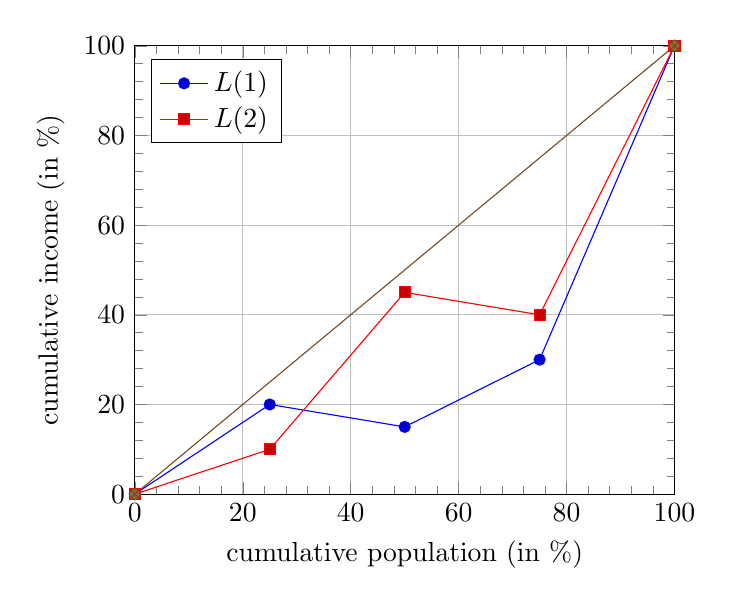
\begin{tikzpicture}
		\begin{axis}[
				xmin=0, xmax=100,
				ymin=0, ymax=100,
				minor tick num = 4,
				grid,
				ylabel = cumulative income (in \%),
				xlabel = cumulative population (in \%),
				legend style={legend pos=north west},
			]
			\addplot plot
			coordinates {(0,0) (25,20) (50,15) (75,30) (100,100)};
			\addplot plot
			coordinates {(0,0) (25,10) (50,45) (75,40) (100,100)};
			\addplot plot [thin]
			coordinates {(0,0) (100,100)};
			\legend{$L(1)$,$L(2)$}
		\end{axis}
	\end{tikzpicture}
\end{frame}

\begin{frame}{Gini Index (CART, IBM IntelligentMiner) (I)}
	\begin{itemize}
		\item Measured impurity of partition $D$ is defined as the sum over $n$ classes:
		      \begin{align*}
			      \text{Gini}(D) = 1-\sum_{j=1}^{n} p_j^2,
		      \end{align*}
		      where $p_j$ is the non-zero probability that sample in $D$ belongs to class $C_j$ as estimated by $\frac{|C_{j,D}|}{|D|}$
		\item If \textbf{attribute $A$ is discrete-valued} with $v$ distinct values
		      compute all possible subsets of values $2^v - 2$. Compute weighted sum of
		      each partition tuble ($D_1$ and $D_2$) as follows:
		      \begin{align*}
			      \text{Gini}_A(D) = \frac{|D_1|}{|D|}\text{Gini}(D_1)+\frac{|D_2|}{|D|}\text{Gini}(D_2).
		      \end{align*}
		\item If \textbf{attribute $A$ is continuous-valued} proceed similarly as in
		      calculating Information Gain for continuous-valued attributes (order values,
		      calculate midpoint of value pairs) and then calculate $\text{Gini}_A(D)$ for
		      every split point.
	\end{itemize}
\end{frame}

\begin{frame}{Gini Index (CART, IBM IntelligentMiner) (II)}
	\begin{itemize}
		\item Gini Index as the \textbf{reduction in impurity} is then given as
		      follows:
		      \begin{align*}
			      \Delta\text{Gini}_A(D) = \text{Gini}(D)-\text{Gini}_A(D).
		      \end{align*}
		\item Attribute with minimum Gini Index is used as the splitting attribute.
	\end{itemize}

\end{frame}

\begin{frame}{Example: Gini Index (I)}
	\begin{itemize}
		\item $D$ has $9$ tuples in $\text{buys\_computer} =$ "yes" and 5 in "no", thus
		      \begin{align*}
			      \text{Gini}(D) = 1 - \left( \frac{9}{14} \right)^2 - \left( \frac{5}{14} \right)^2 = 0.459.
		      \end{align*}
		\item Suppose the attribute $\texttt{income}$ partitions $D$ \\ into $10$ in
		      $D_1:\{\texttt{low,medium}\}$ and $4$ in $D_2: \{\texttt{high}\}$:
		      \begin{align*}
			       & \text{Gini}(D\vert_{D[\texttt{income}]="medium", "low"})                                                                                                                                   \\
			       & = \frac{10}{14} \text{Gini}(D_1) + \frac{4}{14} \text{Gini}(D_2)                                                                                                                           \\
			       & =\frac{10}{14} \left(1-\left( \frac{7}{10} \right)^2 - \left( \frac{3}{10} \right)^2 \right) + \frac{4}{14} \left( 1-\left( \frac{2}{4} \right)^2 - \left( \frac{2}{4} \right)^2 \right) = \\
			       & = 0.443 = \text{gini}(D\vert_{D[\texttt{income}]="high"}).
		      \end{align*}
	\end{itemize}
\end{frame}

\begin{frame}{Computation of Gini Index (II)}
	\begin{itemize}
		\item $\text{Gini}(D\vert_{D[\texttt{income}]="low", "high"}) = 0.458$,\\
		      $\text{Gini}(D\vert_{D[\texttt{income}]="medium", "high"}) = 0.450.$
		\item Thus, split on the \{"low","medium"\} and \{"high"\}, since it has the lowest gini index.
	\end{itemize}
\end{frame}

\begin{frame}{Attribute Selection Measures Overview}
	\textbf{The three measures, in general, return good results, but}
	\begin{itemize}
		\item \textbf{\color{airforceblue}Information Gain:}
		      \begin{itemize}
			      \item Biased towards multi-valued attributes.
		      \end{itemize}
		\item \textbf{\color{airforceblue}Gain Ratio:}
		      \begin{itemize}
			      \item Tends to prefer unbalanced splits in which one partition is much smaller than the others.
		      \end{itemize}
		\item \textbf{\color{airforceblue}Gini Index:}
		      \begin{itemize}
			      \item Biased to multi-valued attributes.
			      \item Has difficulty when number of classes is large.
			      \item Tends to favor tests that result in equal-sized partitions and purity in both partitions.
		      \end{itemize}
	\end{itemize}
\end{frame}

\begin{frame}{Other Attribute Selection Measures}
	\begin{itemize}
		\item \textbf{CHAID:}
		      \begin{itemize}
			      \item A popular Decision-Tree algorithm, measure based on $\chi^2$ test for independence.
		      \end{itemize}
		\item \textbf{C-SEP:}
		      \begin{itemize}
			      \item Performs better than Information Gain and Gini Index in certain cases.
		      \end{itemize}
		\item \textbf{G-statistic:}
		      \begin{itemize}
			      \item Has a close approximation to $\chi^2$ distribution.
		      \end{itemize}
		\item \textbf{MDL (Minimal Description Length) principle:}
		      \begin{itemize}
			      \item I.e. the simplest solution is preferred.
			      \item The best tree is the one that requires the fewest number of bits to both (1) encode the tree and (2) encode the exceptions to the tree.
		      \end{itemize}
		\item \textbf{Multivariate splits:}
		      \begin{itemize}
			      \item Partitioning based on multiple variable combinations.
			      \item CART: finds multivariate splits based on a linear combination of attributes.
		      \end{itemize}
		\item \textbf{Which Attribute Selection Measures is the best?}
		      \begin{itemize}
			      \item Most give good results, none is significantly superior to others.
		      \end{itemize}
	\end{itemize}
\end{frame}

\begin{frame}{Overfitting and Tree Pruning}
	\begin{itemize}
		\item \textbf{Overfitting: An induced tree may overfit the training data.}
		      \begin{itemize}
			      \item Too many branches, some may reflect anomalies due to noise or outliers.
			      \item Poor accuracy for unseen samples.
		      \end{itemize}
		\item Pruned trees are typically smaller, less complex, easier to
		      comprehend, faster and better at classifying unseen data.
		\item \textbf{Two approaches to avoid overfitting:}
		      \begin{enumerate}
			      \item \textbf{\color{airforceblue}Prepruning:}
			            \begin{itemize}
				            \item Halt tree construction early.\\
				                  Do not split a node, if this would result in the goodness measure falling below a threshold.
				            \item Difficult to choose an appropriate threshold.
			            \end{itemize}
			      \item \textbf{\color{airforceblue}Postpruning:}
			            \begin{itemize}
				            \item Remove branches from a "fully grown" tree.\\
				                  Get a sequence of progressively pruned trees.
				            \item Use a set of data different from the training data to decide which is the "best pruned tree."
			            \end{itemize}
		      \end{enumerate}
	\end{itemize}
\end{frame}

\begin{frame}{Enhancements to Basic Decision-Tree Induction}
	\begin{itemize}
		\item \textbf{Allow for} \textbf{\color{airforceblue}continuous-valued attributes.}
		      \begin{itemize}
			      \item Dynamically define new discrete-valued attributes that partition the values of continuous-valued attributes into a discrete set of intervals.
		      \end{itemize}
		\item \textbf{Handle} \textbf{\color{airforceblue}missing attribute values.}
		      \begin{itemize}
			      \item Assign the most common value of the attribute.
			      \item Assign probability to each of the possible values.
		      \end{itemize}
		\item \textbf{\color{airforceblue}Attribute construction.}
		      \begin{itemize}
			      \item Create new attributes based on existing ones that are sparsely represented.
			      \item This reduces fragmentation, repetition, and replication.
		      \end{itemize}
	\end{itemize}
\end{frame}

\begin{frame}{Classification in Large Databases}
	\begin{itemize}
		\item ID3, C4.5, and CART have been developed with the assumption that data fits into memory.\\With Big Data that's not possible anymore.
		\item \textbf{Scalability:}
		      \begin{itemize}
			      \item Classifying datasets with millions of examples and \\ hundreds of attributes with reasonable speed.
		      \end{itemize}
		\item \textbf{Why is decision-tree induction popular?}
		      \begin{itemize}
			      \item Relatively fast learning speed (compared to other classification methods).
			      \item Convertible to simple and easy-to-understand classification rules.
			      \item Can use SQL queries for accessing databases.
			      \item Classification accuracy comparable with other methods.
		      \end{itemize}
		\item Two scalable methods, among others:
		      \begin{enumerate}
			      \item RainForest
			      \item BOAT
		      \end{enumerate}
	\end{itemize}
\end{frame}

\begin{frame}{Scalable Decision Tree: RainForest}
	\begin{itemize}
		\item Applicable to any decision tree algorithm.
		\item \textbf{Separates the scalability aspects from the criteria that determine the quality of the tree.}
		\item \textbf{Builds an} \textbf{\color{airforceblue}AVC-list:} (Attribute, Value, Class\_label).
		\item \textbf{\color{airforceblue}AVC-set} \textbf{(of an attribute X):}
		      \begin{itemize}
			      \item Projection of training dataset onto the attribute $X$ and class label where counts of individual class label are aggregated.
		      \end{itemize}
		\item \textbf{\color{airforceblue}AVC-group} \textbf{(of a node n):}
		      \begin{itemize}
			      \item Set of AVC-sets of all predictor attributes at the node $n$.
		      \end{itemize}
	\end{itemize}
\end{frame}

\begin{frame}{RainForest: Training Set and its AVC-sets}
	\begin{columns}
		\begin{column}{0.6\textwidth}
			\small
			\begin{tabular}{|l|l|c|c|c|}
	\hline
	\rowcolor{faugray!62}\textbf{age} & \textbf{income} & \textbf{student} & \textbf{credit\_rating} & \textbf{buys\_computer} \\\hline
	$\leq 30$                         & high            & no               & fair                    & {\color{faured}no}      \\\hline
	$\leq 30$                         & high            & no               & excellent               & {\color{faured}no}      \\\hline
	$31\ldots40$                      & high            & no               & fair                    & {\color{faugreen}yes}   \\\hline
	$>40$                             & medium          & no               & fair                    & {\color{faugreen}yes}   \\\hline
	$>40$                             & low             & yes              & fair                    & {\color{faugreen}yes}   \\\hline
	$>40$                             & low             & yes              & excellent               & {\color{faured}no}      \\\hline
	$31\ldots40$                      & low             & yes              & excellent               & {\color{faugreen}yes}   \\\hline
	$\leq 30$                         & medium          & no               & fair                    & {\color{faured}no}      \\\hline
	$\leq 30$                         & low             & no               & fair                    & {\color{faugreen}yes}   \\\hline
	$>40$                             & medium          & yes              & fair                    & {\color{faugreen}yes}   \\\hline
	$\leq 30$                         & medium          & yes              & excellent               & {\color{faugreen}yes}   \\\hline
	$31\ldots40$                      & medium          & no               & excellent               & {\color{faugreen}yes}   \\\hline
	$31\ldots40$                      & high            & yes              & fair                    & {\color{faugreen}yes}   \\\hline
	$>40$                             & medium          & no               & excellent               & {\color{faured}no}      \\\hline
\end{tabular}

		\end{column}
		\begin{column}{0.3\textwidth}
			\vspace{-3cm}

			\centering
			AVC-set on age:\\
			\begin{tabular}{|c|c|c|}
				\hline
				age          & yes & no \\\hline
				$\leq 30$    & 2   & 3  \\\hline
				$31\ldots40$ & 4   & 0  \\\hline
				$>40$        & 3   & 2  \\\hline
			\end{tabular}\\[1cm]
			AVC-set on income:\\
			\begin{tabular}{|c|c|c|}
				\hline
				income & yes & no \\\hline
				high   & 2   & 2  \\\hline
				medium & 4   & 2  \\\hline
				low    & 3   & 1  \\\hline
			\end{tabular}
		\end{column}
	\end{columns}
\end{frame}

\begin{frame}{RainForest: Training Set and its AVC-sets (II)}
	\begin{columns}
		\begin{column}{0.6\textwidth}
			\small
			\begin{tabular}{|l|l|c|c|c|}
	\hline
	\rowcolor{faugray!62}\textbf{age} & \textbf{income} & \textbf{student} & \textbf{credit\_rating} & \textbf{buys\_computer} \\\hline
	$\leq 30$                         & high            & no               & fair                    & {\color{faured}no}      \\\hline
	$\leq 30$                         & high            & no               & excellent               & {\color{faured}no}      \\\hline
	$31\ldots40$                      & high            & no               & fair                    & {\color{faugreen}yes}   \\\hline
	$>40$                             & medium          & no               & fair                    & {\color{faugreen}yes}   \\\hline
	$>40$                             & low             & yes              & fair                    & {\color{faugreen}yes}   \\\hline
	$>40$                             & low             & yes              & excellent               & {\color{faured}no}      \\\hline
	$31\ldots40$                      & low             & yes              & excellent               & {\color{faugreen}yes}   \\\hline
	$\leq 30$                         & medium          & no               & fair                    & {\color{faured}no}      \\\hline
	$\leq 30$                         & low             & no               & fair                    & {\color{faugreen}yes}   \\\hline
	$>40$                             & medium          & yes              & fair                    & {\color{faugreen}yes}   \\\hline
	$\leq 30$                         & medium          & yes              & excellent               & {\color{faugreen}yes}   \\\hline
	$31\ldots40$                      & medium          & no               & excellent               & {\color{faugreen}yes}   \\\hline
	$31\ldots40$                      & high            & yes              & fair                    & {\color{faugreen}yes}   \\\hline
	$>40$                             & medium          & no               & excellent               & {\color{faured}no}      \\\hline
\end{tabular}

		\end{column}
		\begin{column}{0.3\textwidth}
			\vspace{-3cm}

			\centering
			AVC-set on student:\\
			\begin{tabular}{|c|c|c|}
				\hline
				student & yes & no \\\hline
				yes     & 6   & 1  \\\hline
				no      & 3   & 4  \\\hline
			\end{tabular}\\[1cm]
			AVC-set on credit\_rating:\\
			\begin{tabular}{|c|c|c|}
				\hline
				credit\_rating & yes & no \\\hline
				fair           & 6   & 2  \\\hline
				excellent      & 3   & 3  \\\hline
			\end{tabular}
		\end{column}
	\end{columns}
\end{frame}

\begin{frame}{Scalable Decision Tree: BOAT}
	\begin{itemize}
		\item BOAT = Bootstrapped Optimistic Algorithm for Tree Construction
		\item \textbf{Use a statistical technique called bootstrapping to create several smaller samples (subsets), each fitting in memory.}
		      \begin{itemize}
			      \item See on the subsequent slides.
		      \end{itemize}
		\item \textbf{Each subset is used to create a tree, resulting in several trees.}
		\item \textbf{These trees are examined and used to construct a new tree T'.}
		      \begin{itemize}
			      \item It turns out that T' is very close to the tree that would be generated \\
			            using the whole data set together.
		      \end{itemize}
		\item \textbf{Advantages:}
		      \begin{itemize}
			      \item Requires only two scans of DB.
			      \item An incremental algorithm:
			            \begin{itemize}
				            \item Take insertions and deletions of training data and update the decision tree.
			            \end{itemize}
		      \end{itemize}
	\end{itemize}
\end{frame}

\begin{frame}{Presentation of Classification Results}
	\centering
	\includegraphics[height=0.8\textheight]{img/classification1.jpeg}
\end{frame}

\begin{frame}{Visualization of a Decision Tree in SGI/MineSet 3.0}
	\centering
	\includegraphics[height=0.8\textheight]{img/classification2.jpeg}
\end{frame}

\begin{frame}{Interactive Visual Mining by Perception-based Classification (PBC)}
	\centering
	\includegraphics[height=0.8\textheight]{img/classification3.jpeg}
\end{frame}
